\documentclass[12pt]{article}
\usepackage{cite}
\usepackage{graphicx}
\usepackage{geometry}
\usepackage{float}
\usepackage{multicol}
\usepackage{subfigure}

\geometry{left=2.0cm,right=2.0cm,top=2.5cm,bottom=2.5cm}

\title{
    \textbf{\Huge ECE385} \\
    \huge Fall 2020 \\
    \huge Experiment 6 \\[120pt]
    \textbf{\Huge Simple Computer SLC-3.2 in SystemVerilog} \\[120pt]
    }

\author{
    \large Name: Zhou Qinren \\ 
            \quad\qquad Zhang Yichi \\
    \large Lab Section: LA3 \\
    \large TA's Name: Yu Yuqi
    }

\date{Nov. $10^{th}$ 2020}

\begin{document}
\setlength{\parindent}{0pt}
\maketitle
\newpage

\section{Introduction}
In this lab, we design and build a simplified version of LC3, SLC3. The SLC3 processor is able to fetch, decode and execute the commands in the SRAM. More specifically speaking, it is able to do basic logical operations, load data from the memory and write data into the memory.

\section{Written Description and Diagrams of SLC-3}
\subsection{Summary of Operation}
This SLC3 controls all its functions by a finite state machine(FSM). The FSM contains three main states, fetch, decode and execute while each state can be more specifically defined as more states. In the fetch state, the processor stores the PC value, the address of the instruction, into the MAR, use this address to get the corresponding instruction and stores it to the MDR which will be passed to IR later. Then in the decode state, the processor will break the instructions down to several parts. The first four bits are opcodes which defines the funtion of this instruction. The rest defines the destination registers(DR), source registers(SR), offsets and some other values needed for the funtions. In the execute state, the specific function is performed. The feasible functions includes ADD, AND, NOT, LDR, STR, BR, JSR, JMP which will be introduced in the next section.

\subsection{Written Description of all .sv Modules}
\begin{figure}[H]
    \centering
    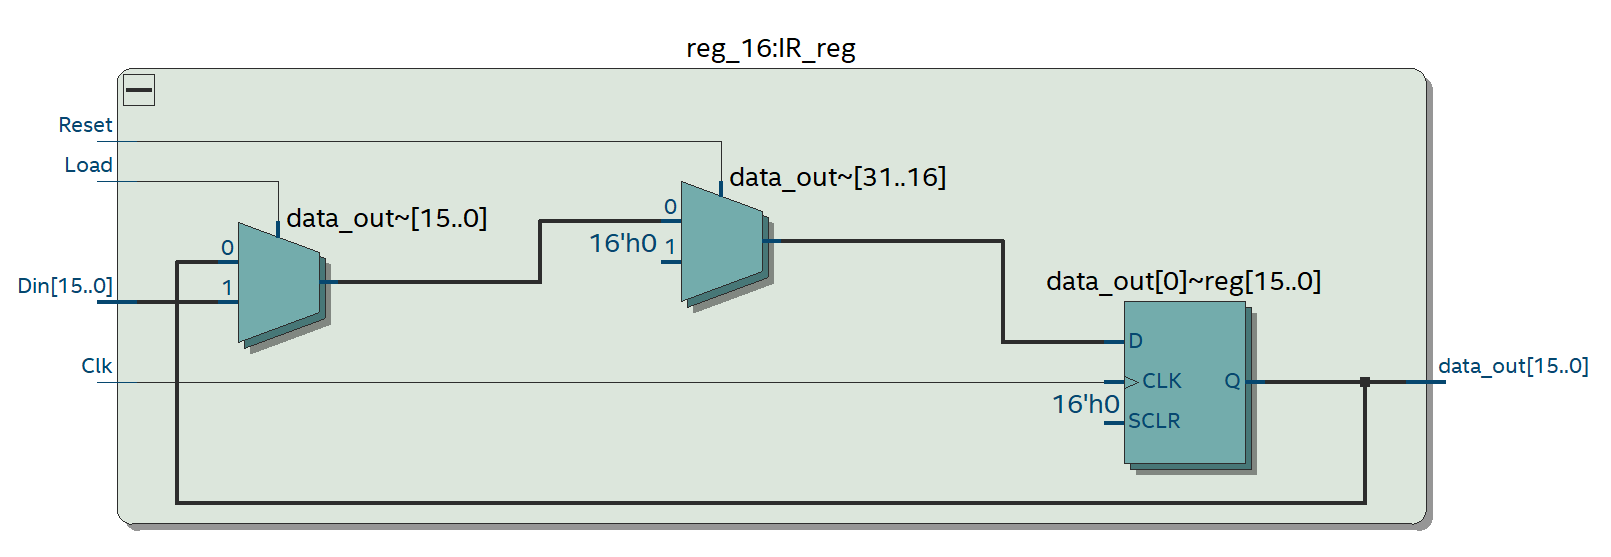
\includegraphics[width=15cm]{reg16.png}
    \caption{Reg\_16.}
\end{figure}
\textbf{Module}: reg\_16 \\ 
\textbf{Inputs}: Clk, Reset, Load, [15:0] Din \\ 
\textbf{Outputs}: [15:0] data\_Out \\ 
\textbf{Description}: This is a positive-edge triggered 16-bit register with synchronous reset, load. \\ 
\textbf{Purpose}: This module is a register unit which will be used to store the PC, MAR, MDR and IR values. \\

\begin{figure}[H]
    \centering
    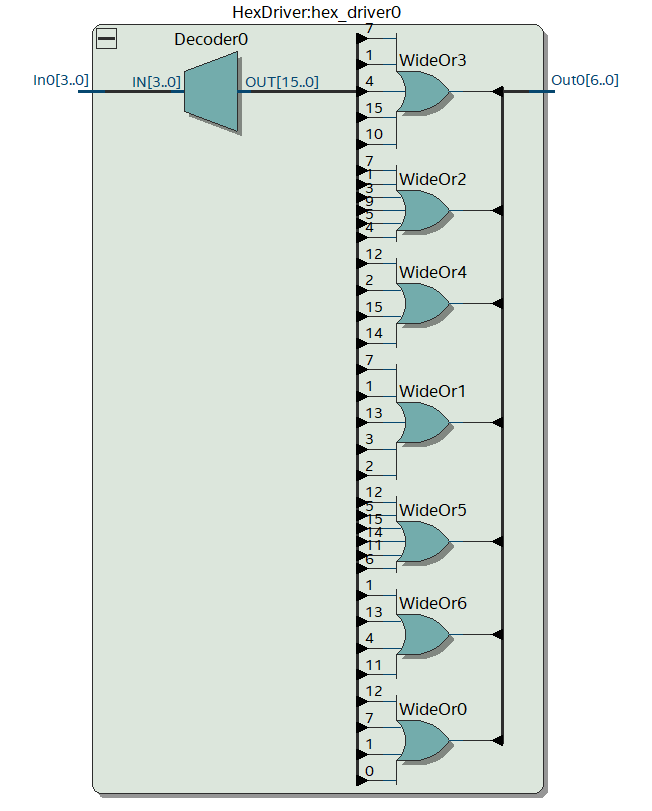
\includegraphics[width=8cm]{hexdriver.png}
    \caption{HexDriver.}
\end{figure}
\textbf{Module}: HexDriver \\ 
\textbf{Inputs}: [3:0] In0\\ 
\textbf{Outputs}: [6:0] Out0\\ 
\textbf{Description}: The HexDriver module takes in a 4-bit number and outputs its corresponding 7-bit number representing a hex number (one of "0123456789ABCDEF"). \\ 
\textbf{Purpose}: HexDriver turns the result 4-bit number to its corresponding hex number for FPGA to show on the digital monitor. \\

\begin{figure}[H]
    \centering
    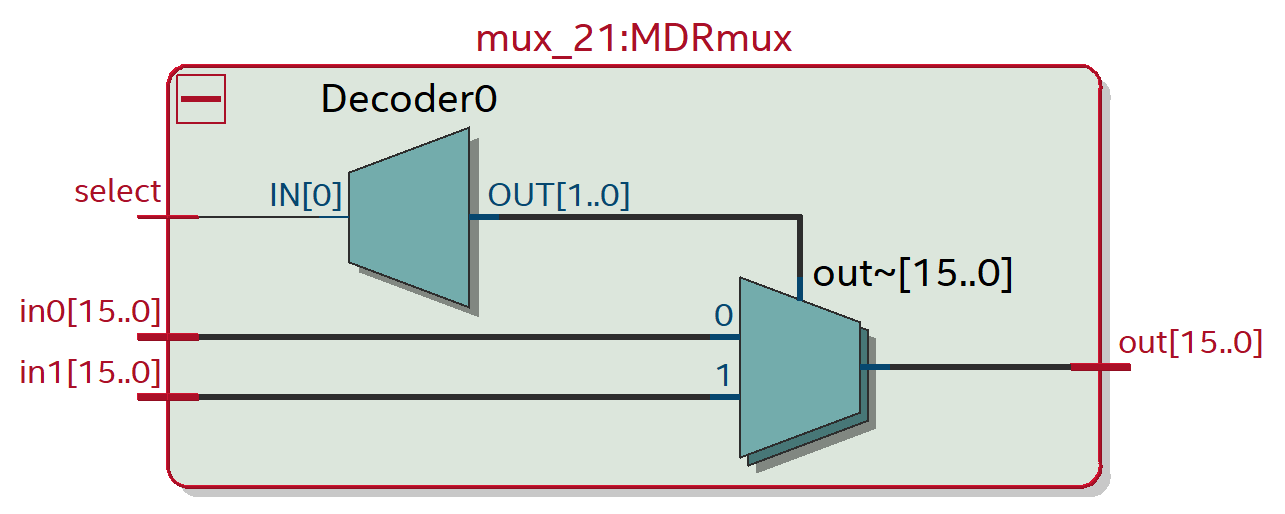
\includegraphics[width=15cm]{mux21.png}
    \caption{Mux\_21.}
\end{figure}
\textbf{Module}: mux\_21 \\ 
\textbf{Inputs}: select, [N-1:0] in0, [N-1:0] in1\\ 
\textbf{Outputs}: [N-1:0] out\\ 
\textbf{Description}: This is a dynamic 2-to-1 mux that can take two N bits signals then select and output the one we want. \\ 
\textbf{Purpose}: This kind of mux is used for DRmux, SR1mux, SR2mux, ADDR1mux and MDRmux. \\

\begin{figure}[H]
    \centering
    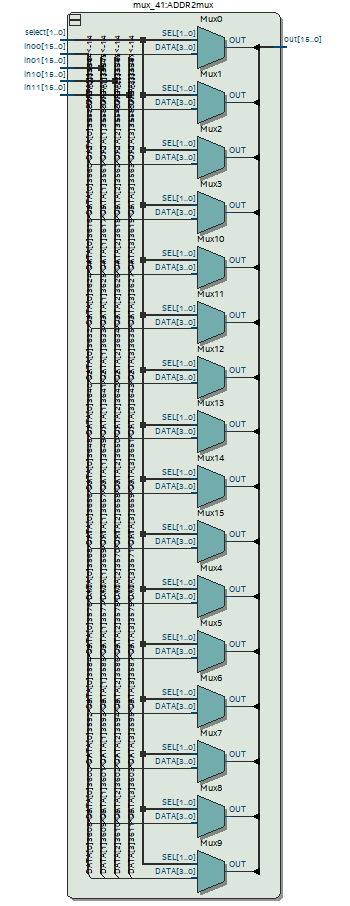
\includegraphics[width=6cm]{mux41.png}
    \caption{Mux\_41.}
\end{figure}
\textbf{Module}: mux\_41 \\ 
\textbf{Inputs}: [1:0] select, [N-1:0] in00, [N-1:0] in01, [N-1:0] in10, [N-1:0] in11 \\ 
\textbf{Outputs}: [N-1:0] out\\ 
\textbf{Description}: This is a dynamic 4-to-1 mux that can take four N bits signals then select and output the one we want. \\ 
\textbf{Purpose}: This kind of mux is used for PCmux and ADDR2mux. \\

\begin{figure}[H]
    \centering
    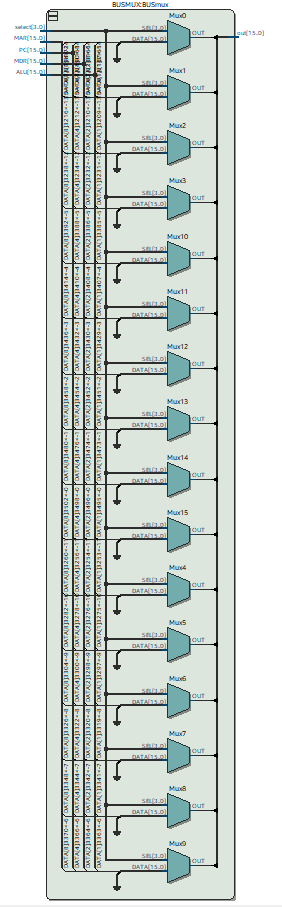
\includegraphics[width=6cm]{busmux.png}
    \caption{BUSMUX.}
\end{figure}
\textbf{Module}: BUSMUX \\ 
\textbf{Inputs}: [3:0] select, MAR, PC, MDR, ALU\\ 
\textbf{Outputs}: [N-1:0] out\\ 
\textbf{Description}: This is a 4-to-1 mux with one-hot encoding that takes four signals then select and output the one we want. One select signal corresponds to one specific input signal. \\ 
\textbf{Purpose}: This is a replacement of tristate buffers since the FPGA does not support internal tristate buffers. It selects which signal to be passed to the bus. \\

\begin{figure}[H]
    \centering
    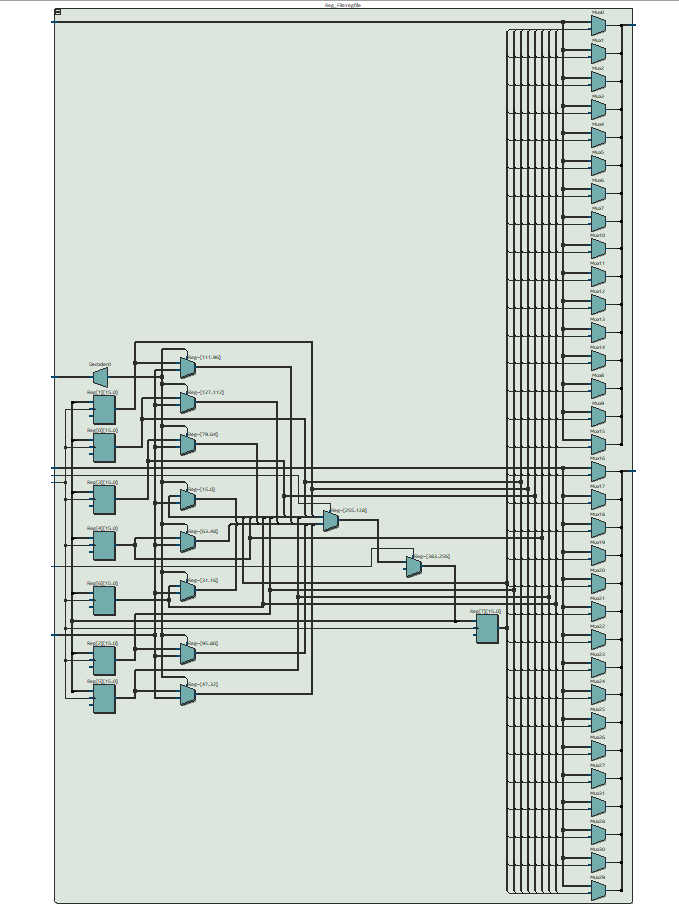
\includegraphics[width=8cm]{regfiles.png}
    \caption{Reg\_File.}
\end{figure}
\textbf{Module}: Reg\_File \\ 
\textbf{Inputs}: [2:0] SR1, [2:0] SR2, [2:0] DR, [15:0] BUS, Clk, Reset, LD\_REG\\ 
\textbf{Outputs}: [15:0] SR1OUT, [15:0] SR2OUT\\ 
\textbf{Description}: This is the combination of 8 16-bits registers that can take the values from the bus. \\ 
\textbf{Purpose}: This is a temporary small memory to store the value to be calculated, used or stored to the memory. It can speed up the process since reading from and writing into memory is relatively slow. \\

\begin{figure}[H]
    \centering
    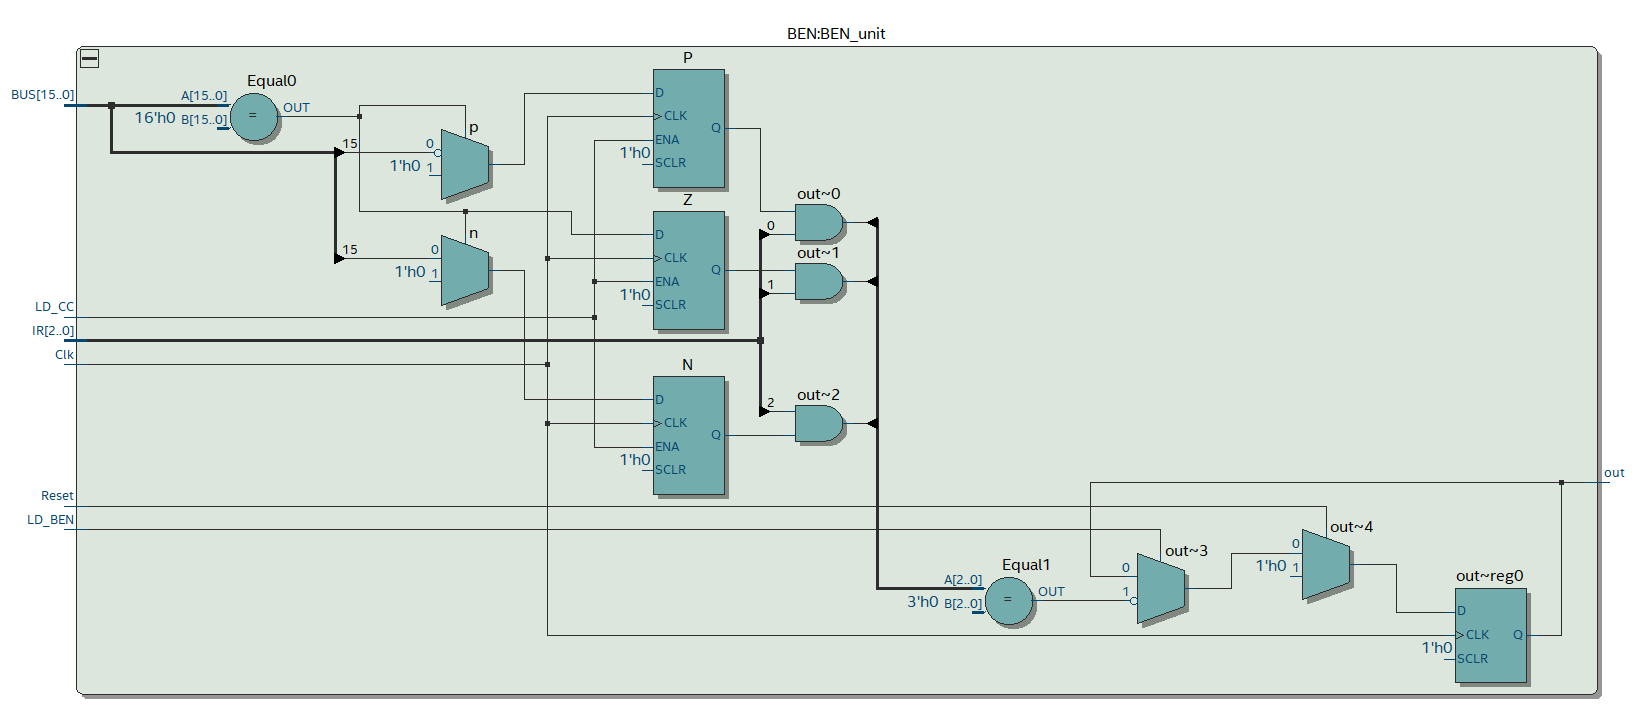
\includegraphics[width=15cm]{ben.png}
    \caption{BEN.}
\end{figure}
\textbf{Module}: BEN \\ 
\textbf{Inputs}: [2:0] IR, [15:0] BUS, LD\_BEN, LD\_CC, Clk, Reset\\ 
\textbf{Outputs}: out \\ 
\textbf{Description}: This is a register that stores the sign of the values operated before (positive, negative or zero) and outputs whether the sign matches the nzp that is input from the branch instruction. \\
\textbf{Purpose}: This is specifically designed for the branch instruction to help check whether it meets the condition to branch. \\

\begin{figure}[H]
    \centering
    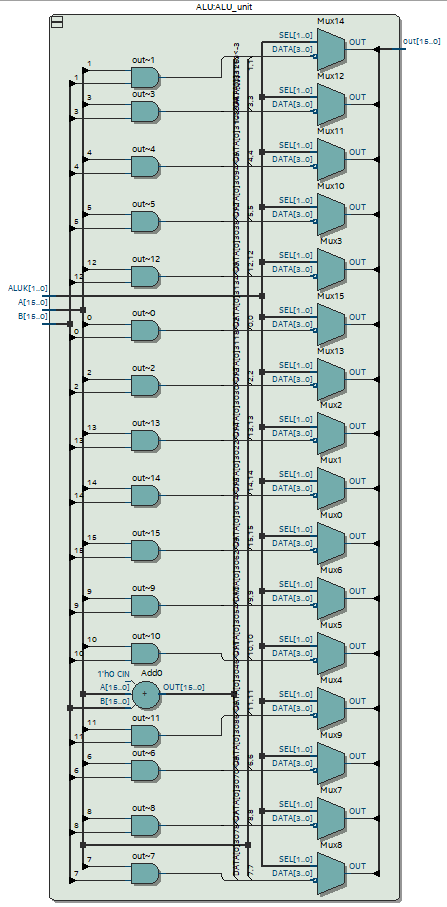
\includegraphics[width=6cm]{alu.png}
    \caption{ALU.}
\end{figure}
\textbf{Module}: ALU \\ 
\textbf{Inputs}: [15:0] A, [15:0] B, [1:0] ALUK \\ 
\textbf{Outputs}: [15:0] out \\ 
\textbf{Description}: This unit takes two inputs, calculates with desired funtion and outputs the result. \\
\textbf{Purpose}: This is an Arithmetic Logic Unit that does the computation. \\

\begin{figure}[H]
    \centering
    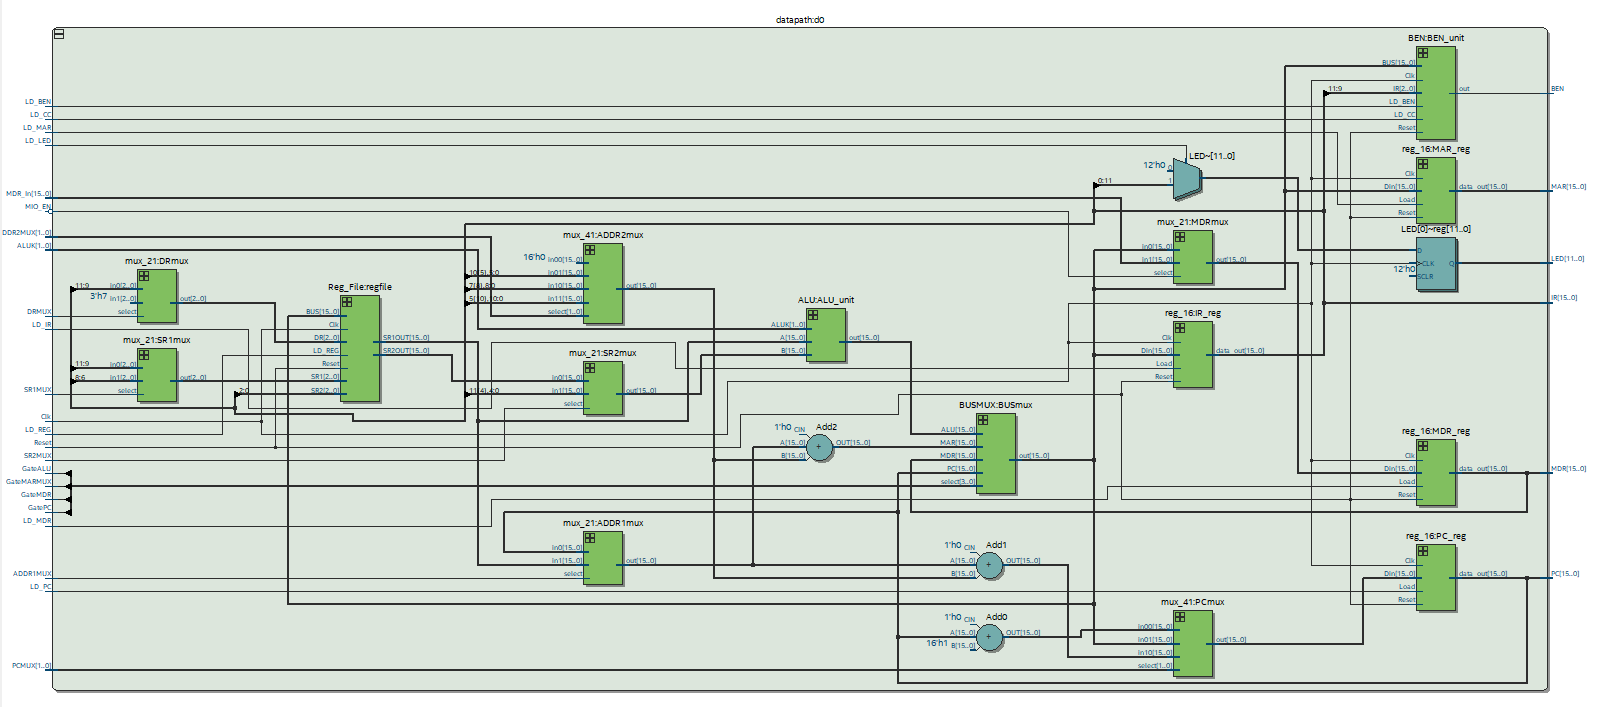
\includegraphics[width=15cm]{datapath.png}
    \caption{Datapath.}
\end{figure}
\textbf{Module}: datapath \\ 
\textbf{Inputs}: Clk, Reset, GatePC, GateMDR, GateALU, GateMARMUX, LD\_MAR, LD\_MDR, LD\_IR, LD\_BEN, LD\_CC, LD\_REG, LD\_PC, LD\_LED, [1:0] PCMUX, [1:0] ADDR2MUX, [1:0] ALUK, DRMUX, SR1MUX, SR2MUX, ADDR1MUX, MIO\_EN, [15:0] MDR\_In\\ 
\textbf{Outputs}: [15:0] MAR, [15:0] MDR, [15:0] IR, [15:0] PC, BEN, [11:0] LED \\ 
\textbf{Description}: This unit connects PC, MAR, MDR, BEN, ALU, control unit and Reg\_File and pass data among them. \\
\textbf{Purpose}: This is the datapath of the SLC3 that transfers PC, MAR, MDR, IR, specifically, addresses, data to be computed and data to be stored. \\

\begin{figure}[H]
    \centering
    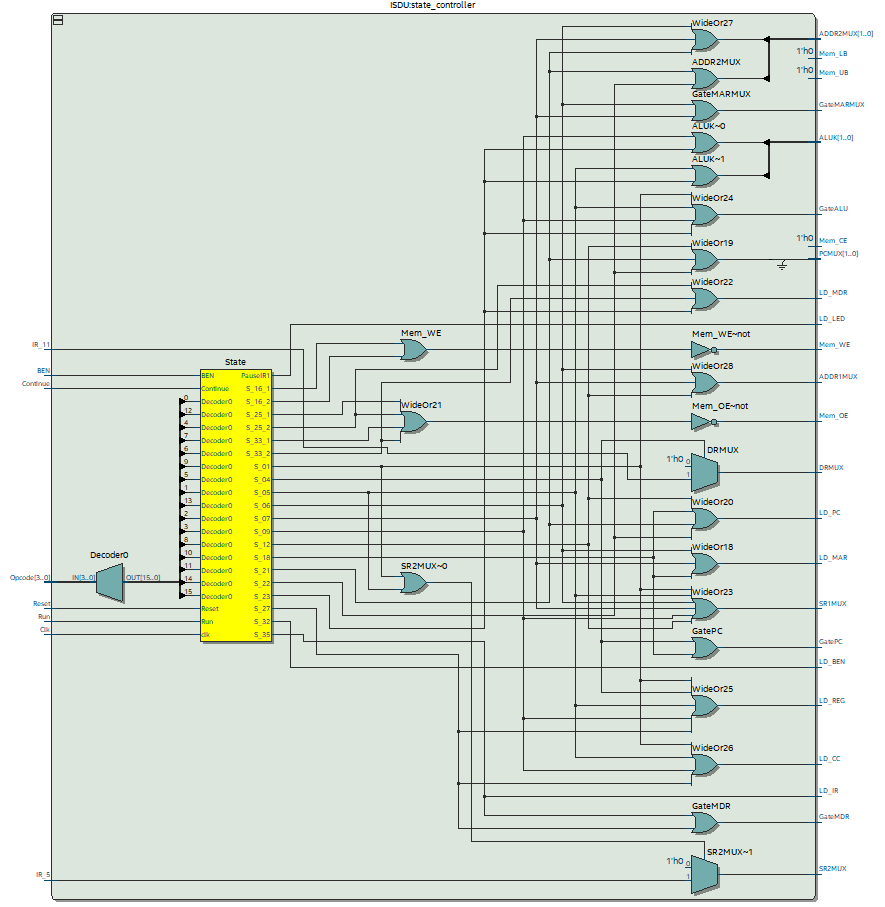
\includegraphics[width=15cm]{ISDU.png}
    \caption{ISDU.}
\end{figure}
\textbf{Module}: ISDU \\ 
\textbf{Inputs}: Clk, Reset, Run, Continue, [3:0] Opcode,[N-1:0], IR\_5, IR\_11, BEN \\ 
\textbf{Outputs}: GatePC, GateMDR, GateALU, GateMARMUX, LD\_MAR, LD\_MDR, LD\_IR, LD\_BEN, LD\_CC, LD\_REG, LD\_PC, LD\_LED, [1:0] PCMUX, [1:0] ADDR2MUX, [1:0] ALUK, DRMUX, SR1MUX, SR2MUX, ADDR1MUX, Mem\_CE, Mem\_UB, Mem\_LB, Mem\_OE, Mem\_WE \\ 
\textbf{Description}: This is an FSM with states that performs FETCH, DECODE, ADD, AND, NOT, LDR, STR, BR, JSR, JMP, PAUSE and HALT. \\
\textbf{Purpose}: This is an FSM with 24 states that controls what the SLC3 do (fetch, decode, pause or execute the functions). \\

\begin{figure}[H]
    \centering
    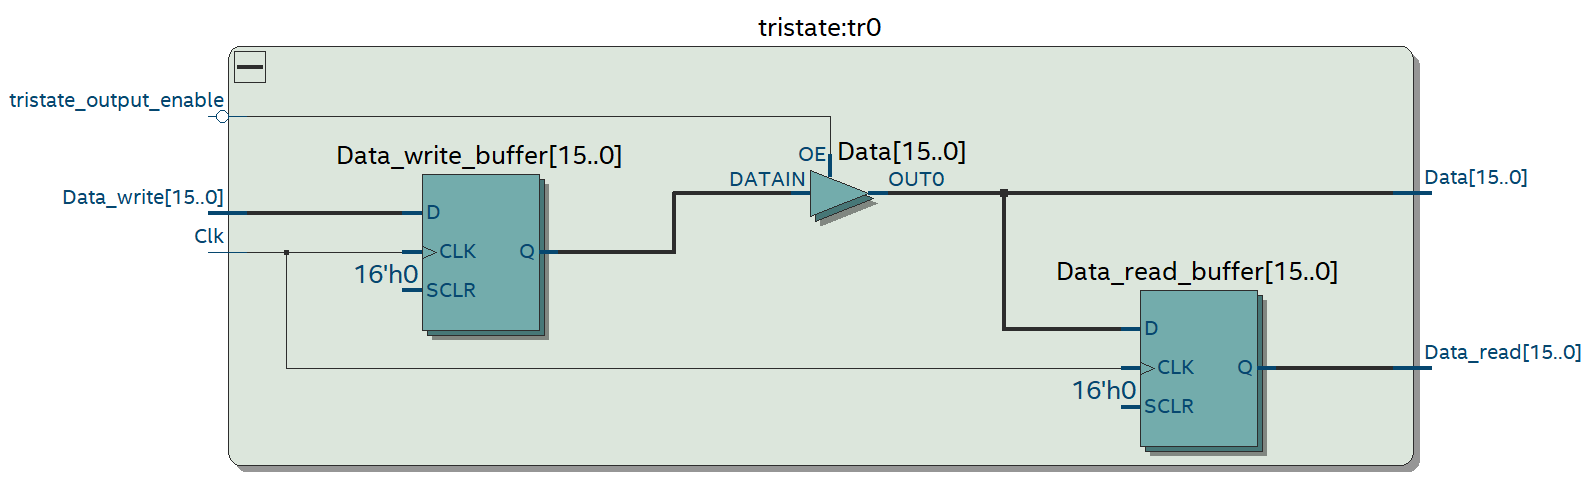
\includegraphics[width=15cm]{tristate.png}
    \caption{Tristate.}
\end{figure}
\textbf{Module}: tristate \\ 
\textbf{Inputs}: Clk, tristate\_output\_enable, [N-1:0] Data\_write \\ 
\textbf{Outputs}: [N-1:0] Data\_read \\ 
\textbf{Inouts}: [N-1:0] Data \\
\textbf{Description}: This unit exchanges data between SRAM and datapath. \\
\textbf{Purpose}: This is a tristate buffer that helps to protect the data. \\

\textbf{Module}: test\_memory \\ 
\textbf{Inputs}: Clk, Reset, [15:0] I\_O, [19:0] A, CE, UB, LB, OE, WE \\ 
\textbf{Description}: This is a simulated memory. \\
\textbf{Purpose}: This is only used for simulation. It performs similar to the SRAM on the DE2 board. \\

\textbf{Module}: sync \\ 
\textbf{Inputs}: Clk, d \\ 
\textbf{Outputs}: q \\ 
\textbf{Description}: Synchronize the inputs with no reset. \\
\textbf{Purpose}: Synchronizer for switches and buttons. \\

\textbf{Module}: sync\_r0 \\ 
\textbf{Inputs}: Clk, Reset, d \\ 
\textbf{Outputs}: q \\ 
\textbf{Description}: Synchronize the inputs with reset to 0. \\
\textbf{Purpose}: Synchronizer for D-flipflop. \\

\textbf{Module}: sync\_r0 \\ 
\textbf{Inputs}: Clk, Reset, d \\ 
\textbf{Outputs}: q \\ 
\textbf{Description}: Synchronize the inputs with reset to 0. \\
\textbf{Purpose}: Synchronizer for D-flipflop. \\

\textbf{Module}: sync\_r1 \\ 
\textbf{Inputs}: Clk, Reset, d \\ 
\textbf{Outputs}: q \\ 
\textbf{Description}: Synchronize the inputs with reset to 1. \\
\textbf{Purpose}: Synchronizer for D-flipflop. \\

\textbf{Module}: slc3 \\ 
\textbf{Inputs}: [15:0] S, Clk, Reset, Run, Continue \\ 
\textbf{Outputs}: [11:0] LED, [6:0] HEX0, [6:0] HEX1, [6:0] HEX2, [6:0] HEX3, [6:0] HEX4, [6:0] HEX5, [6:0] HEX6, [6:0] HEX7, CE, UB, LB, OE, WE, [19:0] ADDR \\ 
\textbf{Inouts}: [15:0] Data \\
\textbf{Description}: This module connects the memory, datapath, ISDU, and hexdrivers. \\
\textbf{Purpose}: This is the entire SLC3. \\

\begin{figure}[H]
    \centering
    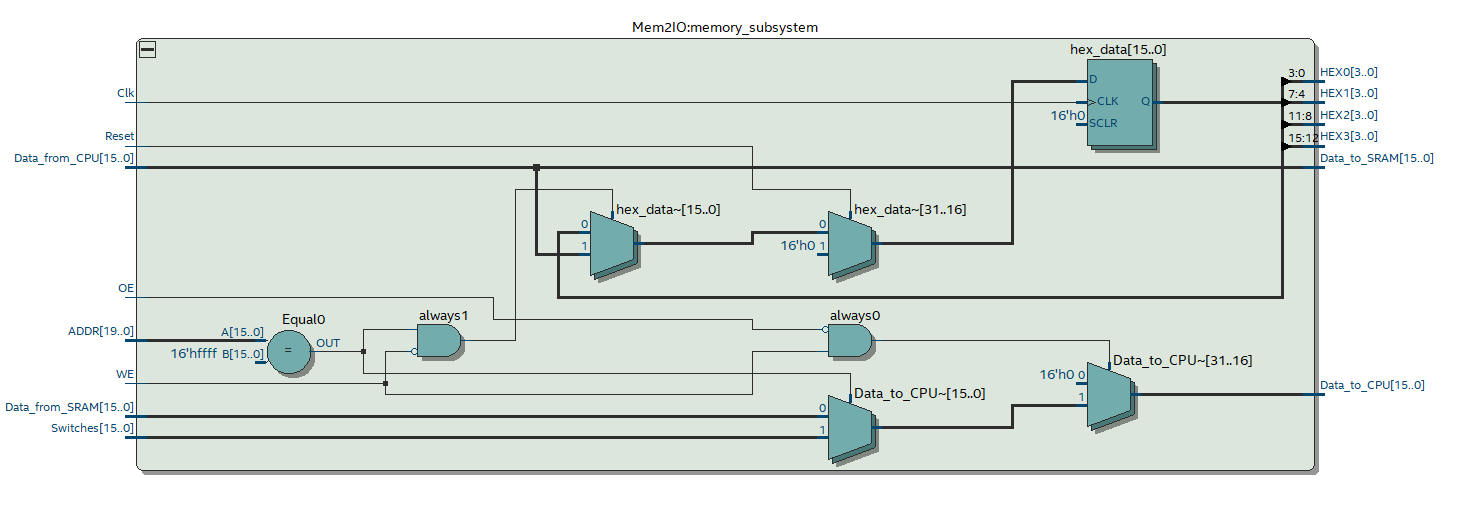
\includegraphics[width=15cm]{mem2IO.png}
    \caption{Mem2IO.}
\end{figure}
\textbf{Module}: Mem2IO \\ 
\textbf{Inputs}: CE, UB, LB, OE, WE, [19:0] ADDR, [15:0] Switches, Clk, Reset, [15:0] Data\_from\_CPU, [15:0]   Data\_from\_SRAM \\ 
\textbf{Outputs}: [15:0] Data\_to\_CPU, [15:0] Data\_to\_SRAM, [3:0] HEX0, [3:0] HEX1, [3:0] HEX2, [3:0] HEX3 \\ 
\textbf{Description}: This module connects the memory, datapath, LEDs,  switches and hexdrivers. \\
\textbf{Purpose}: This module controls the data between the CPU and the SRAM and the inputs (switches) and the outputs (LEDs). \\

\subsection{Block Diagram of slc3.sv
}
\begin{figure}[H]
    \centering
    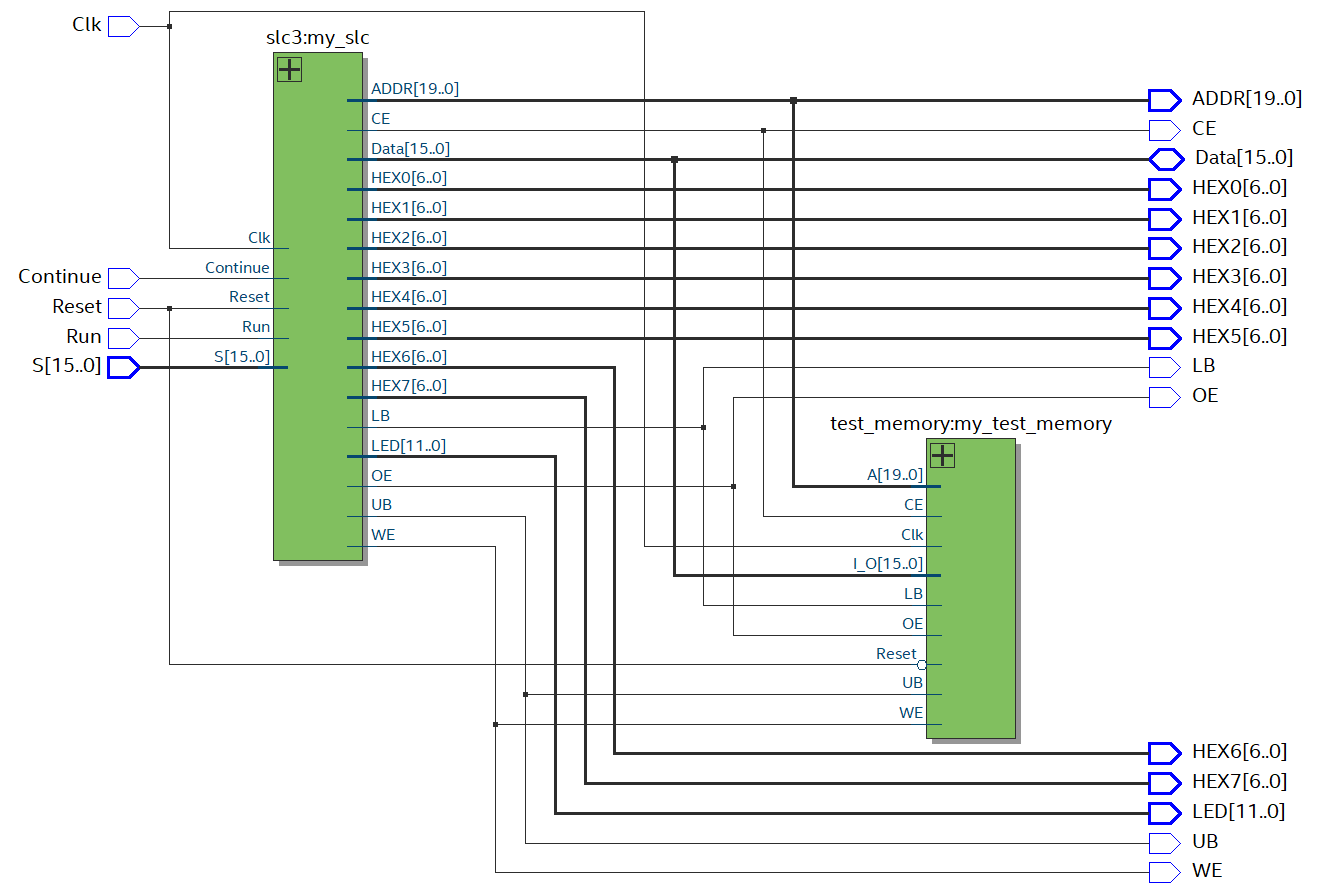
\includegraphics[width=15cm]{SLC3.png}
    \caption{The block diagram of slc3.}
\end{figure}

\subsection{Description of the operation of the ISDU (Instruction Sequence Decoder Unit)}
ISDU is essentially a finite state machine. It generates several outputs, which can be divided into three groups: Load, Gate and Mux Select. Load is used to load the corresponding register. Gate is used to indicate which data should be connected to the bus. Mux select is used to select the input of the corresponding mux, such as the operands of ALU and the register address in register file. ISDU also deals with the memory via some memory control signal connected to MEM2IO. \\

After IR loads the newest instruction, the transition leads to DECODE state. Then state machine goes to different states based on the instruction. For example, if the instruction is ADD, the next state is state 1. ISDU will output the corresponding MUX Select signal to choose the destination register and source register. Moreover, ISDU will choose the operands of ALU. It will also output LD\_REG, LD\_CC and Gate\_ALU. 

\subsection{State Diagram of ISDU
}
\begin{figure}[H]
    \centering
    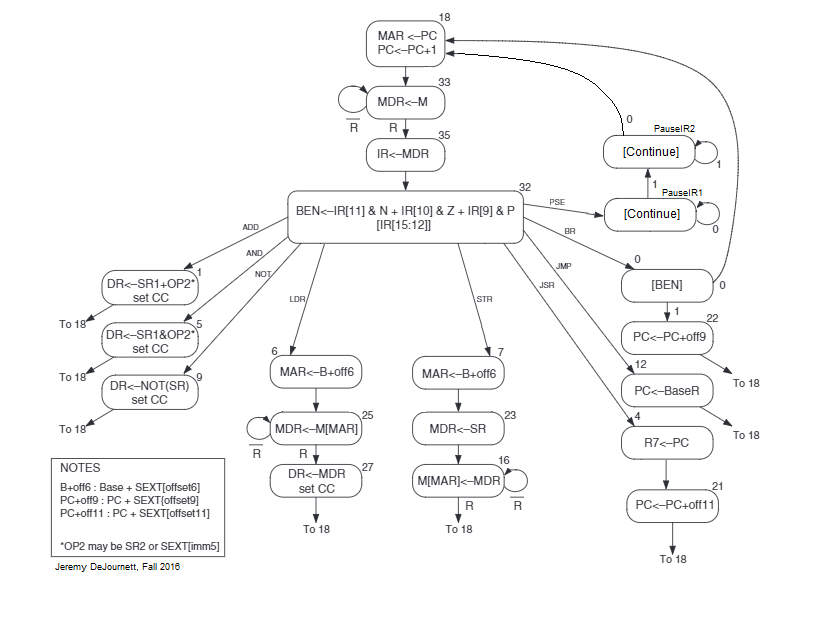
\includegraphics[width=15cm]{states.png}
    \caption{The state diagram of ISDU.}
\end{figure}

\section{Simulations of SLC-3 Instructions}
\begin{figure}[H]
    \centering
    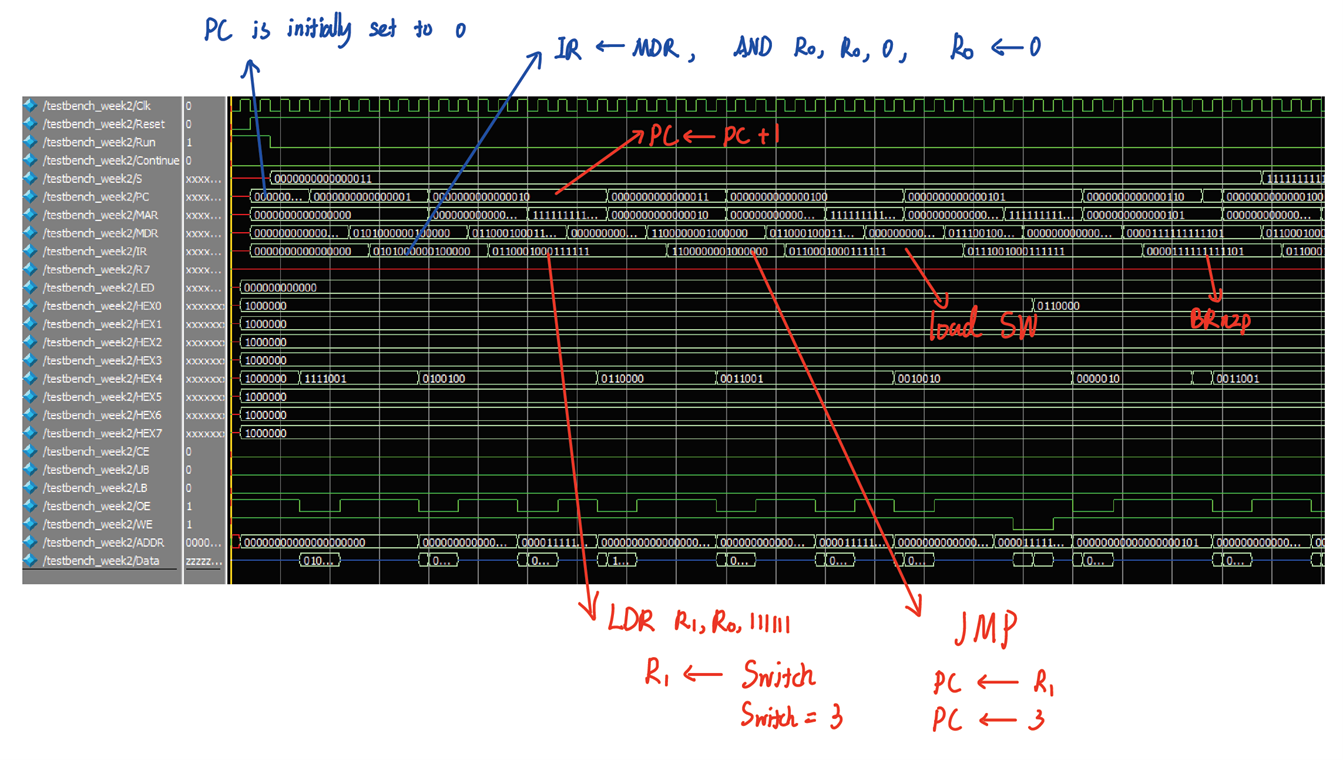
\includegraphics[width=15cm]{simulation.png}
    \caption{The simulations of SLC-3 instructions.}
\end{figure}

\section{Post-Lab Questions}
\begin{table}[H]
    \centering
    \resizebox*{9cm}{6cm}{
        \begin{tabular}{|l|l|l|l|}
        \hline
        LUT           & 593        \\ \hline
        DSP           & 0          \\ \hline
        Memory        & 0          \\ \hline
        Flip-Flop     & 280        \\ \hline
        Frequency     & 65.11MHz   \\ \hline
        Static Power  & 98.66mW    \\ \hline
        Dynamic Power & 8.54mW     \\ \hline
        Total Power   & 179.18mW   \\ \hline
        \end{tabular}
    }
    \caption{Design statistics table for the multiplier.}
\end{table}

Questions: What is the function of the MEM2IO.sv module? \\

Answers: MEM2IO is the interface between the memory and control unit. It can also deal with the switch input. The control unit generates some control signals to interact with the MEM2IO, which will handle the data transition between the memory. \\

Questions: What is the difference between the BR and JMP instructions? \\

BR is conditional jump; it will change PC if the condition code nzp is satisfied. JMP is unconditional jump; PC will certainly change when executing the instruction. \\

Questions: What is the purpose of the R signal in Patt and Patel? How do we compensate for the lack of the signal in our design? What implications does this have for synchronization? \\

Answers: R signal is used to indicate that the memory is ready for read / write operation. In our design, we found that the memory will be ready in two cycles under any circumstances, thus, we assigned two states for each read or write operation. We don’t have to use synchronizers, since we use states to control the memory.

\section{Conclusion}
\subsection{Functionality}
Our design is a small computer, which is capable of performing several instructions, such as ADD, AND, NOT, BR, JMP, JSR, LDR, STR, and PAUSE. The computer can read input from the switch and store data into memory. It can also perform some mathematical operation between two operands. 
\subsection{About Lab Manual}
We are looking forward to have more materials about the FPGA, e.g. the chips on it, how it works, etc.

\newpage
\bibliography{}
\bibliographystyle{ieeetr}
\end{document}